% =============================================================================
% File      : ex_doc_2-26.tex -- example 2.26
% Author    : Jürgen Hackl <hackl.j@gmx.at>
% Creation  : 2019-08-14
% Time-stamp: <Wed 2019-08-14 17:04 juergen>
%
% Copyright (c) 2019 Jürgen Hackl <hackl.j@gmx.at>
% =============================================================================
\documentclass{standalone}
\usepackage{../../tikz-network}
\begin{document}
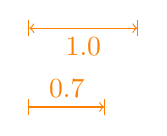
\begin{tikzpicture}
  \Vertex{A} \Vertex[x=2]{B}
  \Edge[label=X,distance=.7](A)(B)
  \draw[orange,|->|] (.3,-.5) --++ (0.98,0) node[pos=.5,above]{$0.7$};
  \draw[orange,|<->|] (.3,.5) --++ (1.4,0) node[pos=.5,below]{$1.0$};
\end{tikzpicture}
\end{document}
% =============================================================================
% eof

%%% Local Variables:
%%% mode: latex
%%% TeX-master: t
%%% End:
